\chapter{Gait Generation and Optimization for Modular Robots}
  This chapter will discuss the application of the PDABGA in a gait-optimization
    scenario involving three connected modular robots.
  

\section{Gait Implementation}
  A novel gait control method has been implemented for usage on the Mobot.
  The Mobot has several limitations which prevent the usage of some of the
    high-tech cutting edge gait control laws which have been used for some
    other multi-jointed robots. 
  Specifically, the Mobot can only communicate via Bluetooth and lacks the
    capability of forming Bluetooth piconets. 
  This means that Mobots cannot communicate directly with each other, and
    cooperating Mobots must communicate with a central computational device,
    such as a computer, tablet, or smartphone. 
  Furthermore, the bandwidth of the communication channel is fairly limited.
  These limitations preclude the usage of any gait control method that 
    requires fast communication across modules, such as the majority of 
    distributed gaits and neural nets.

  Therefore, the gait implementation chosen for this research, based on
    previous work done by Yang et. al. \cite{Yang2006}, requires no 
    inter-module communication and very little central control, needing
    only a synchronizing clock from the central controller to function.
  At the same time, the gait implementation is very expressive compared to
    some more primitive gait implementations, such as gait tables.
  It can also theoretically implement any periodic gait, and is easily
    optimizable evolutionary algorithms.
  This is accomplished by representing the motion of each joint of a gait 
    as a list of Fourier series coefficients. 
  The infinite Fourier series, shown in Equation \ref{eq:fourier}, is a
    representation of any periodic function as a summation of sin and 
    cosine functions.

  \begin{equation}
  \label{eq:fourier}
  f(t) = \frac{1}{2} a_0 + 
  \sum_{i=1}^{\infty} a_i \sin\left(\frac{2 \pi i}{T}t\right) + 
  \sum_{i=1}^{\infty} b_i \cos\left(\frac{2 \pi i}{T}t\right)
  \end{equation}
  
  The Mobots used for this research have been augmented with a Fourier series
    control law, shown in Figure \ref{fig:motor_controller_architecture}.
  Basically, the implementation is a Fourier series function generator which
    produces a stream of angle values depending on the current local time and the 
    currently stored Fourier series coefficients.
  The PID controller drives the motor to the best of its ability to follow 
    the signal provided by the Fourier series function generator.
  Note that almost the entire implementation and execution of the Fourier series
    gait happens locally on the robot.
  There are only two extra-modular communication events which need to occur to 
    run a Fourier series based gait.
    \begin{itemize}
      \item First, the central controller needs to modify the stored Fourier series 
        coefficients on each robot. This step is not time critical and may be 
        performed in series over the list of connected robots.
      \item Second, the central controller needs to issue a synchronizition
        signal to all of the robots, acting like a starting gun to start the
        robotic gait. Ideally, this signal should be sent in parallel to each
        robot simultaneously to perfectly synchronize their clocks, but 
        fundamental limitations with Bluetooth prevent this. However,
        the communication events occur on a timescale magnitudes of order
        shorter than robotic motions and thus any delay caused by this step
        are deemed negligable. When each robot receives the synchronization
        signal, it stores it's own current clock time, $t_c$ which is the
        number of milliseconds since the robot has powered on, into a 
        variable $t_s$. The function generator then uses the value
        $(t_c - t_s)$ as the time value in the Fourier series function generator,
        thus synchronizing the function generators across multiple modules.
    \end{itemize}
  
  % FIGURE --------------------------------------------------
  \begin{figure}[!ht]
  \begin{center}
     \includegraphics[width=5in]{figures/motor_controller_architecture}
  \end{center}
  \caption{\label{fig:motor_controller_architecture}Standard Mobot
  motor controller augmented with Fourier series function generator.}
  \end{figure}
  % END FIG -------------------------------------------------

\section{Simulation Design}

\section{Chromosome Design}

